\documentclass[tikz,border=8pt]{standalone}
\usepackage{amsmath}
\usetikzlibrary{arrows.meta,positioning,fit,backgrounds,calc}
\definecolor{maroon}{RGB}{128,0,0}
\definecolor{paper}{RGB}{250,247,243}
\definecolor{inkgray}{RGB}{110,96,98}
\begin{document}
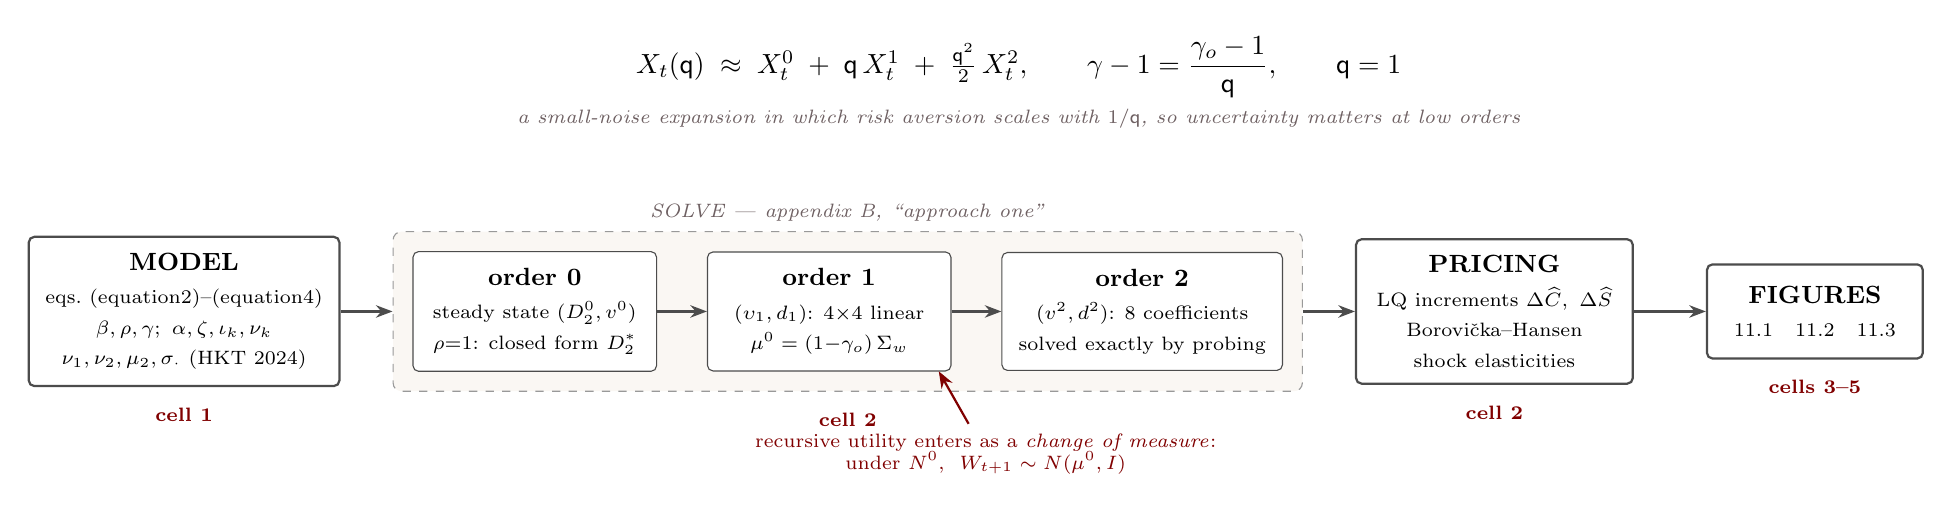
\begin{tikzpicture}[
  font=\small,
  box/.style={draw=black!70, rounded corners=2pt, align=center,
              inner sep=6pt, minimum height=34pt, fill=white},
  stage/.style={box, thick},
  order/.style={box, minimum width=88pt},
  lbl/.style={font=\scriptsize\itshape, text=inkgray},
  cell/.style={font=\scriptsize\bfseries, text=maroon},
  arr/.style={-{Stealth[length=6pt]}, thick, black!70},
  note/.style={font=\scriptsize, text=maroon, align=center}]

% ---------- headline: the expansion ----------
\node[font=\normalsize, align=center] (headline) at (10.6, 3.1)
  {$X_t(\mathsf q)\;\approx\;X_t^0 \;+\; \mathsf q\,X_t^1 \;+\;
    \tfrac{\mathsf q^2}{2}\,X_t^2, \qquad
    \gamma-1=\dfrac{\gamma_o-1}{\mathsf q}, \qquad \mathsf q=1$};
\node[lbl] at (10.6, 2.45)
  {a small-noise expansion in which risk aversion scales with $1/\mathsf q$,
   so uncertainty matters at low orders};

% ---------- flow ----------
\node[stage, minimum width=95pt] (model) at (0,0)
  {\textbf{MODEL}\\[1pt]
   \scriptsize eqs.\ (equation2)--(equation4)\\
   \scriptsize $\beta,\rho,\gamma;\ \alpha,\zeta,\iota_k,\nu_k$\\
   \scriptsize $\nu_1,\nu_2,\mu_2,\sigma_\cdot$ (HKT 2024)};

\node[order, right=26pt of model] (o0)
  {\textbf{order 0}\\[1pt]\scriptsize steady state $(D_2^0, v^0)$\\
   \scriptsize $\rho{=}1$: closed form $D_2^*$};
\node[order, right=18pt of o0] (o1)
  {\textbf{order 1}\\[1pt]\scriptsize $(\upsilon_1, d_1)$: $4{\times}4$ linear\\
   \scriptsize $\mu^0=(1{-}\gamma_o)\,\Sigma_w$};
\node[order, right=18pt of o1] (o2)
  {\textbf{order 2}\\[1pt]\scriptsize $(v^2, d^2)$: 8 coefficients\\
   \scriptsize solved exactly by probing};

\node[stage, right=26pt of o2, minimum width=100pt] (price)
  {\textbf{PRICING}\\[1pt]
   \scriptsize LQ increments $\Delta\widehat C,\ \Delta\widehat S$\\
   \scriptsize Borovi\v{c}ka--Hansen\\ \scriptsize shock elasticities};

\node[stage, right=26pt of price, minimum width=78pt] (figs)
  {\textbf{FIGURES}\\[1pt]\scriptsize 11.1\quad 11.2\quad 11.3};

\begin{scope}[on background layer]
\node[draw=black!40, dashed, rounded corners=3pt, inner sep=7pt,
      fill=paper, fit=(o0)(o1)(o2)] (solvebox) {};
\end{scope}
\node[lbl, anchor=south] at (solvebox.north) {SOLVE — appendix B, ``approach one''};

\draw[arr] (model) -- (solvebox.west|-model);
\draw[arr] (o0) -- (o1);
\draw[arr] (o1) -- (o2);
\draw[arr] (solvebox.east|-model) -- (price);
\draw[arr] (price) -- (figs);

% ---------- the N^0 measure annotation ----------
\node[note] (n0) at ($(o1.south)!0.5!(o2.south) + (0,-1.05)$)
  {recursive utility enters as a \emph{change of measure}:\\
   under $N^0$,\ \ $W_{t+1}\sim N(\mu^0, I)$};
\draw[arr, maroon] (n0) -- ($(o1.south)!0.35!(o2.south)$);

% ---------- cell mapping ----------
\node[cell, anchor=north] at ($(model.south)+(0,-4pt)$)   {cell 1};
\node[cell, anchor=north] at ($(solvebox.south)+(0,-4pt)$){cell 2};
\node[cell, anchor=north] at ($(price.south)+(0,-4pt)$)   {cell 2};
\node[cell, anchor=north] at ($(figs.south)+(0,-4pt)$)    {cells 3--5};
\end{tikzpicture}
\end{document}
